% -----------------------------*- LaTeX -*------------------------------
\documentclass[12pt]{report}
\usepackage{%
	amsfonts,%
	amsmath,%	
	amssymb,%
	amsthm,%
	algorithm,%
	babel,%
	bbm,%
	etex,%
	%biblatex,%
	caption,%
	centernot,%
	color,%
	dsfont,%
	enumerate,%
	epsfig,%
	epstopdf,%
	geometry,%
	graphicx,%
	hyperref,%
	latexsym,%
	mathtools,%
	multicol,%
	pgf,%
	pgfplots,%
	pgfplotstable,%
	pgfpages,%
	proof,%
	psfrag,%
	subfigure,%	
	tikz,%
	ulem,%
	url%
}	
\usepackage[noend]{algpseudocode}
\usepackage[mathscr]{eucal}
\usepgflibrary{shapes}
\usetikzlibrary{%
  	arrows,%
	backgrounds,%
	chains,%
	decorations.pathmorphing,% /pgf/decoration/random steps | erste Graphik
	decorations.text,%
	matrix,%
  	positioning,% wg. " of "
  	fit,%
	patterns,%
  	petri,%
	plotmarks,%
  	scopes,%
	shadows,%
  	shapes.misc,% wg. rounded rectangle
  	shapes.arrows,%
	shapes.callouts,%
  	shapes%
}

\theoremstyle{plain}
\newtheorem{thm}{Theorem}[section]
\newtheorem{lem}[thm]{Lemma}
\newtheorem{prop}[thm]{Proposition}
\newtheorem{cor}[thm]{Corollary}

\theoremstyle{definition}
\newtheorem{defn}[thm]{Definition}
\newtheorem{conj}[thm]{Conjecture}
\newtheorem{exmp}[thm]{Example}
\newtheorem{assum}[thm]{Assumptions}
\newtheorem{axiom}[thm]{Axiom}

\theoremstyle{remark}
\newtheorem{rem}{Remark}
\newtheorem{note}{Note}
\newtheorem{fact}{Fact}

\newcommand{\norm}[1]{\left\lVert#1\right\rVert}
\newcommand{\indep}{\!\perp\!\!\!\perp}
\DeclarePairedDelimiter\abs{\lvert}{\rvert}%
\newcommand\numberthis{\addtocounter{equation}{1}\tag{\theequation}}
\newcommand{\tr}{\operatorname{tr}}
\newcommand{\R}{\mathbb{R}}
\newcommand{\N}{\mathbb{N}}
\newcommand{\E}{\mathbb{E}}
\newcommand{\Z}{\mathbb{Z}}
\newcommand{\B}{\mathscr{B}}
\newcommand{\C}{\mathcal{C}}
\newcommand{\T}{\mathscr{T}}
\newcommand{\F}{\mathcal{F}}
\newcommand{\G}{\mathcal{G}}
%\newcommand{\ba}{\begin{align*}}
%\newcommand{\ea}{\end{align*}}
\DeclareMathOperator*{\argmax}{arg\,max}
\renewcommand{\qedsymbol}{$\blacksquare$}
\makeatletter
\def\BState{\State\hskip-\ALG@thistlm}
\makeatother

\makeatletter
\def\th@plain{%
  \thm@notefont{}% same as heading font
  \itshape % body font
}
\def\th@definition{%
  \thm@notefont{}% same as heading font
  \normalfont % body font
}
\makeatother
\date{}
\usepackage{scribe_e1244}
\usepackage{times}
\begin{document}


\lecturer{Aditya Gopalan}		% optional, put lecturer's name here
\scribe{Anantha Narayanan R, Ashok D R}		% required, put your name here
\lecturenumber{3}			% required, must be a number
\lecturedate{September 10}		% required, omit year
\maketitle

% ----------------------------------------------------------------------

\section{Recap}

In the last class, we discussed binary hypotheses testing under Bayesian hypotheses testing framework. Bayesian hypotheses testing framework assumes that the hypothesis pair $H_0$ and $H_1$ have prior probabilities $\pi_0$ and $\pi_1$ respectively. We determined the general form for the optimal decision rule under this setup for given cost structure ($C_{ij}$). As an application, the optimal decision rule for the ``Location testing problem with Gaussian error" was determined.

%--------------------------------------------------------

\section{Introduction to MiniMax Hypothesis Testing}

The Bayesian Optimal Rule $\delta$ is a decision rule that minimises the Bayes Risk $r(\delta)$ {\em given the prior probabilities} for the hypothesis $H_0$ and $H_1$ as $\pi_0$ and $\pi_1$ respectively. But, who gives the prior probabilities? What is the guarantee that the prior probabilities are accurate? What can we do without assuming prior probabilities $(\pi_0,1-\pi_0)$. One way to address this issue, when the prior probabilities are not available, is to use the {\bf Minimax hypothesis testing} Framework.

\subsection{Minimax Hypothesis Testing Framework}
This framework seeks to determine the decision rule $\delta^*$ that minimises the maximum cost. In other words, the Minimax optimal rule is defined as,

\begin{align*}
	\delta^{*} &\bydef \arg \min_{\delta} \max(R_0(\delta),R_1(\delta)) \\
	&\bydef \arg \min_{\delta} \max_{j\in\{0,1\}}(R_j(\delta))
\end{align*}


\begin{rem} : Another way to think of the above framework is to assume $\pi_0 = 0$ or $\pi_1 = 0$ in the Bayes hypotheses testing setup. But this is pessimistic in a way because, consider 2 decision rules $\delta_1$ and $\delta_2$ with the conditional risks $(R_0(\delta),R_1(\delta)))$ being $(0.01,10)$ and $(9,10)$ respectively.\\ We can see that $\max(0.01,10) = \max(9,10) = 10$. Thus, this framework is not satisfactory as according to Minimax hypotheses testing criteria both the decision rules $\delta_1$ and $\delta_2$ are equally optimal (we know that, trivially $\delta_1$ is the better decision rule).
\end{rem}
			
	\subsection{How to find the Minimax Rule?}
	The quantities given to us for determining the Minimax decision rule are the observation space ($\Gamma$), the probability distributions associated with the hypotheses pair $H_0$ and $H_1$ which are $\mathbb{P}_0$ and $\mathbb{P}_1$ respectively, and the cost structure ($C_{ij}$).\\
	
	\noindent The decision rule,
	\begin{align*}
		\delta^* = \arg \min_{\delta} \max_{j\in \{0,1\}}(R_j(\delta)).
	\end{align*}
	\\
	This can be re-written as,
	\begin{align}
		\delta^* = \arg \min_{\delta} \max_{\pi_0 \in [0,1]} (\pi_0 R_0(\delta) \: + \: (1-\pi_0) R_1(\delta)).
	\end{align}

	\noindent Remark: The term inside the {\bf Max} expression can be thought of as a smooth straight line running from $R_1(\delta)$ to $R_0(\delta)$. The maximum value of that line will be one of the extremity of the line, i.e. either $R_1(\delta)$ or $R_0(\delta)$(Figure \ref{fig:BayesLine}).\\
	


	\begin{figure}[htbp]
		\begin{center}
			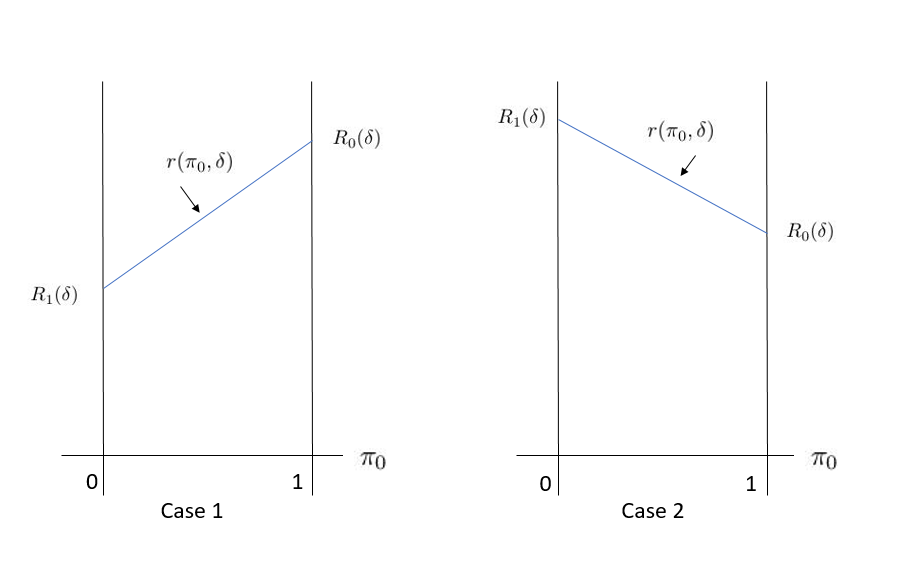
\includegraphics[scale = 0.39]{Figures/BayesLine.png}
			\caption{Plots to depict that the extremes are the maximum in a linear function}
			\label{fig:BayesLine}
		\end{center}
	\end{figure}

	
	
	\noindent Let us define the Bayes risk as follows,
	\begin{align}
	r(\pi_0,\delta) \bydef \pi_0 R_0(\delta) \: + \: (1-\pi_0) R_1(\delta).
	\end{align}
	
	\noindent Thus the Minimax optimal decision rule can be written as,

	\begin{align}
	\delta^* =	\arg \min_{\delta} \max_{\pi_0 \in \{0,1\}} r(\pi_0,\delta).
	\end{align}

	
	\subsubsection{Minimax Inequality}
	Statement : Given a Function
	\begin{align*}
		f \: : \: A \times B \to \mathbb{R},
	\end{align*}
	
	\noindent it can be shown that,
	\begin{align*}
		\min_{b} \max_{a} f(a,b) \geq \max_{a} \min_{b} f(a,b) \: \: \: \: \forall \: a \in A, b \in B.
	\end{align*}

	\noindent The above inequality is called the Minimax inequality.

 
	\noindent Using the Minimax Inequality and from equation (3.1), we get,
	
	\begin{align*}
		\min_{\delta} \max_{\pi_0 \in [0,1]} r(\pi_0,\delta) \geq \max_{\pi_0 \in [0,1]} \min_{\delta} r(\pi_0,\delta).
	\end{align*}
	
	\noindent The inner optimisation of the RHS $\min_\delta r(\pi_0,\delta)$, is nothing but the Bayes optimality problem.\\
	
	\noindent Let us define,
	\begin{align*}
		V(\pi_0) = r(\pi_0,\delta_{\pi_0}) = \min_{\delta} r(\pi_0,\delta)
	\end{align*}
	
	where $\delta_{\pi_0} \to$ Bayes optimal rule for prior $\pi_0$.\\
	
	\noindent Thus we get,
	\begin{align}
		\min_{\delta} \max_{\pi_0 \in [0,1]} r(\pi_0,\delta) \geq \max_{\pi_0 \in [0,1]} V(\pi_0).
	\end{align}

\subsubsection{Wishful Thinking}

Perhaps we can find $\pi_L$ such that it maximises $V(.)$, and claim that its Bayes optimal rule $\delta_{\pi_L}$ is Minimax optimal.\\

\noindent Recollect that $r(\pi_0,\delta_{\pi_x})$ is a smooth line from $R_1(\delta_{\pi_x})$ to $R_0(\delta_{\pi_x})$. For different values of $\pi_x \in [0,1]$, we get infinitely many lines (Figure \ref{fig:bayesrisklines}).

%diagram of lines
\begin{figure}[htbp]
	\begin{center}
		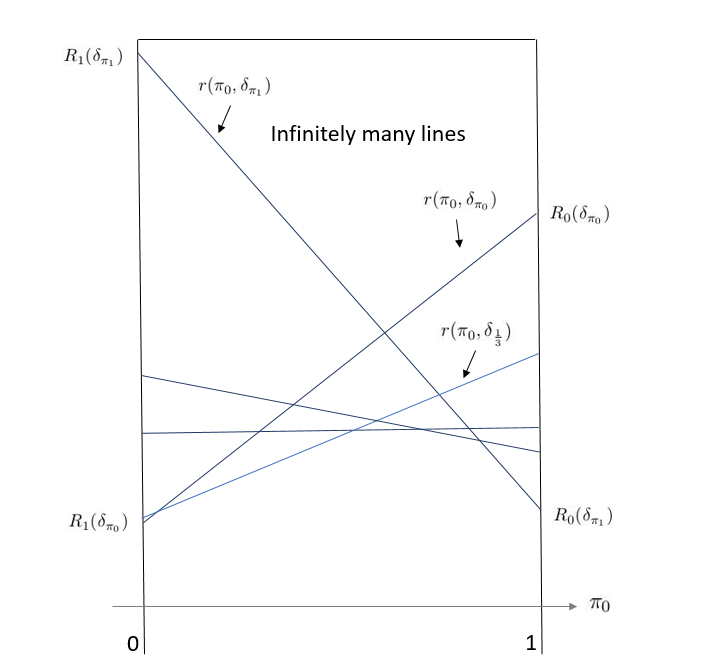
\includegraphics[scale = 0.5]{Figures/BayesRiskLines.png}
		\caption{Plot depicting the Bayes risk values for different decision rules $\delta$ vs $\pi_0$}
		\label{fig:bayesrisklines}
	\end{center}
\end{figure}

\newpage 
\noindent Since V(.) is the minimum of the linear functions, the plot of V(.) vs $\pi_0$ is a convace function on the interval $[0,1]$ (Figure \ref{fig:wishfulthinking}).

% diagram of v(.)
\begin{figure}[htbp]
	\begin{center}
		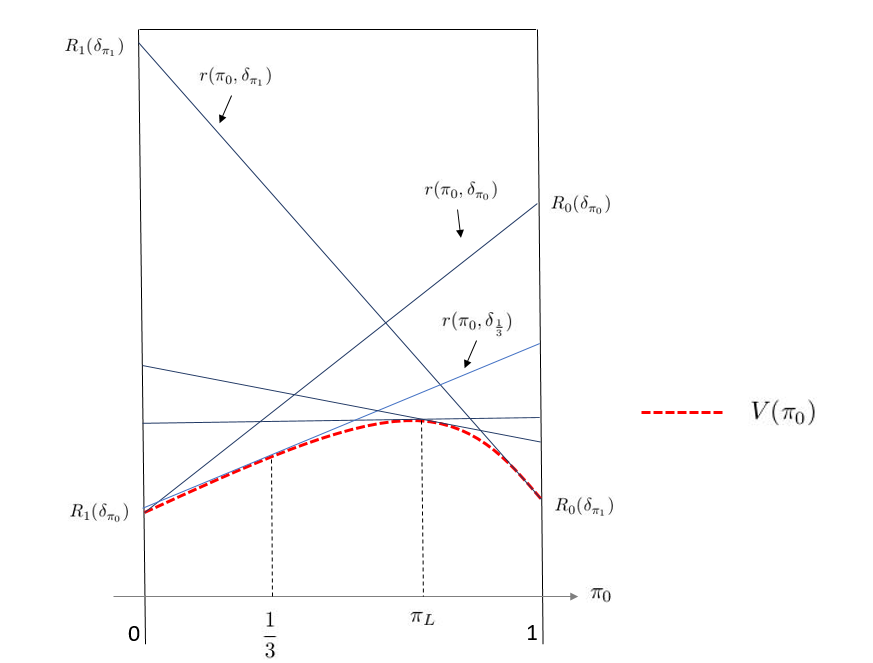
\includegraphics[scale = 0.4]{Figures/WishfulThinking.png}
		\caption{Plot of $V(\pi_0)$}
		\label{fig:wishfulthinking}
	\end{center}
\end{figure}




\noindent (Note: A function $f : [a,b] \to \mathbb{R}$ is concave if $f(\lambda x + (1-\lambda) y) \geq \lambda f(x) + (1-\lambda) f(y)$, \: $\forall x,y \in [a,b]$ and $\lambda \in [0,1]$.)\\

\noindent We observe that at $\pi_0 = \pi_L$, $V(\pi_0)$ is maximum. The slope of the tangent at $V(\pi_L)$ is zero. Thus we can say that $R_0(\delta_{\pi_L})$ = $R_1(\delta_{\pi_L})$ (Figure \ref{fig:BayesisMinimax}).

\begin{figure}[htbp]
	\begin{center}
		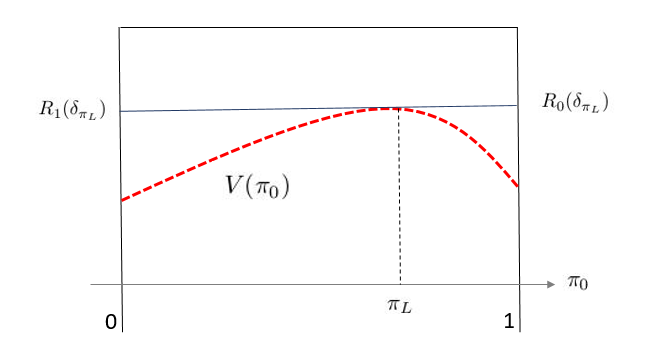
\includegraphics[scale = 0.6]{Figures/BayesisMinimax.png}
		\caption{Bayes Decision Rule $\delta_{\pi_L}$ is Minimax}
		\label{fig:BayesisMinimax}
	\end{center}
\end{figure}

\newpage
\noindent Thus pictorially for any other decision rule $\delta$ we have,
\begin{align*}
	\max_{j \in \{0,1\}}R_j(\delta) \geq R_0(\delta_{\pi_L}).
\end{align*}

\noindent This can be intuitively understood as for any point of the right of $\pi_L$, $R_1(\delta)$ will move above  $R_1(\delta_{\pi_L})$, and for any point to the left of $\pi_L$, $R_0(\delta)$ will move above  $R_0(\delta_{\pi_L})$.\\

\noindent Also, analytically since the min-max meets the lower bound for the prior $\pi_L$ and the associated $\delta_{\pi_L}$ decision rule, Minimax decision rule is Bayes decision rule for the prior $\pi_L$.\\
\noindent {\bf  Wishful thinking makes sense!!!} 
\section{Structure of minimax rules}
\begin{thm}\label{thm minimax rules}

Suppose $\pi_L \in [0,1]$ maximizes the function V over [0,1], i.e, $V(\pi_L)=\displaystyle{ \max_{\pi_0\in [0,1]}} \, V(\pi_0)$. Moreover, suppose one of the following conditions holds:-
\begin{enumerate}
\item $\pi_L=0$.
\item $\pi_L=1$.
\item $R_0({\delta_{\pi_L}}) \, = \,R_1({\delta_{\pi_L}})$, for some Bayes rule $\delta_{\pi_L}$ corresponding to $\pi_L$.
\end{enumerate}
Then, $\delta{\pi_L}$ is a minimax rule.
i.e, $\max \{R_0({\delta_{\pi_L}}) \, , \,R_1({\delta_{\pi_L}})\} \, \leq \, \max \{R_0(\delta) \, , \, R_1(\delta) \} \, \forall \, \delta$.
\end{thm}

\begin{rem}

 $\pi_L$ is called a ``Least favourable prior". 

\end{rem}

\begin{proof}
\begin{itemize}

    \item {\underline{Case 3:}} In this case the risk $r$ as a function of prior will be constant and therefore independent of the prior.  i.e,
    \begin{align*}
         \,r(\pi_0,\delta_{\pi_L})\, &= \, r(\pi_L,\delta_{\pi_L}),\, \forall \, \pi_0 \in [0,1], \\
         \displaystyle{\max_{\pi_0 \in[0,1]}} \, r(\pi_0,\delta_{\pi_L})\, &= \, r(\pi_L,\delta_{\pi_L}) \, = \, V(\pi_L).  \numberthis \label{eqn1}
    \end{align*}
    And we know from the definition of $\pi_L$,
    \begin{align*}
        V(\pi_L) \, &= \, \displaystyle{\max_{\pi_0'}} \, V(\pi_0'),\\
        V(\pi_L) \, &= \, \displaystyle{\max_{\pi_0'}} \, \displaystyle{\min_\delta} \, r(\pi_0',\delta),\\
        \displaystyle{\max_{\pi_0 \in [0,1]}} \, r(\pi_0,\delta_{\pi_L}) \, &= \, \displaystyle{\max_{\pi_0'}} \, \displaystyle{\min_\delta} \, r(\pi_0',\delta), \, (\text{ From \, \ref{eqn1} })\\
        \displaystyle{\min_\delta} \, \displaystyle{\max_{\pi_0 \in [0,1]}} \, r(\pi_0,\delta) \, & \leq \,  \displaystyle{\max_{\pi_0'}} \, \displaystyle{\min_\delta} \, r(\pi_0',\delta).\numberthis \label{eqn2}
    \end{align*}
    Thus from the Minimax inequality and eqn \ref{eqn2}, we have,   
    \begin{align*}
        \,\displaystyle{\min_\delta} \, \displaystyle{\max_{\pi_0 \in [0,1]}} \, r(\pi_0,\delta) \, &= \, \displaystyle{\max_{\pi_0'}} \, \displaystyle{\min_\delta} \, r(\pi_0',\delta),\\
        \displaystyle{\min_\delta} \, \displaystyle{\max_{\pi_0 \in [0,1]}} \, r(\pi_0,\delta) \, &= \,V(\pi_L) \, = \, r(\pi_L,\delta_{\pi_L}).
    \end{align*}
    Hence in this case $\delta_{\pi_L}$ is the Minimax decision rule.
    
    \item {\underline{Case 1}}:- $\pi_L=0$ or $V(0) \, \geq \, V(\pi_0) \, \forall \, \pi_0 \in [0,1]$.
    
    \begin{figure}[htbp]
    \begin{center}
    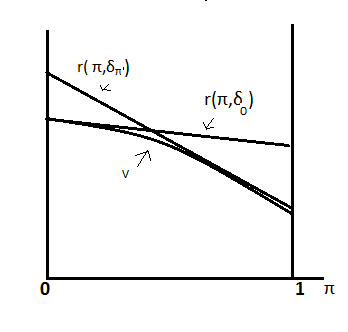
\includegraphics[scale = 0.8]{Figures/case1.png}
    \caption{Plot of V function for case 1 }
    \label{fig: V function }
    \end{center}
    \end{figure}
    
    In this case $ r(\pi_0,\delta_0)$ is tangent to $V(\pi_0)$ at $0$. Since $V(\pi_0)$ is maximum at $0$, we must have slope of tangent $\leq \, 0$ $\forall \, \pi_0 \in[0,1]$, which implies  $R_1(\delta_0)  \geq  R_0(\delta_0)$. Thus, 
    
    \begin{align*}
        R_1(\delta_0) \, &= \max \, \{ R_1(\delta_0) \, , \, R_0(\delta_0) \},\\
        &= \, \displaystyle{\max_{\pi_0\in [0,1]}} \, r(\pi_0, \delta_0),\\
        R_1(\delta_0) \, & \geq \, \displaystyle{\min_{\delta}} \, \displaystyle{\max_{\pi_0\in [0,1]}} \, r(\pi_0, \delta_0).\numberthis \label{eqn3}\\
    \end{align*}
    
    Again from the Minimax inequality and from eqn \ref{eqn3}, we have, 
        $$R_1(\delta_0) \, = \, V(0) \, = \, \displaystyle{\min_{\delta}} \, \displaystyle{\max_{\pi_0\in [0,1]}} \, r(\pi_0, \delta_0).$$
    Hence $\delta_0$ is the Minimax decision rule in this case and the prior $\pi_0 = 0$ is the maximizer of the V function.
    
    \item {\underline{Case 2}}:- $\pi_L=0$.
    
    On similar lines to case 1, in this case, we will get $\delta_1$ as the Minimax decision rule and the prior $\pi_0 = 1$ as the maximizer of the V function.
\end{itemize}
\end{proof}

The Theorem \ref{thm minimax rules} can be summarized by the following tree diagram:-

\tikzstyle{Box} = [rectangle, minimum width=3cm, minimum height=1cm, text centered, draw=white, fill=white]
\tikzstyle{arrow} = [thick,->,>=stealth]

\begin{tikzpicture}[node distance=2cm]

\node(Box1) [Box] {$\pi_L\in\{0,1\}$};
\node(Box2) [Box, xshift=5cm, yshift=3cm]{$\pi_L$ : Maximizer of $V$ function};
\node(Box3) [Box, xshift=9cm]{$\pi_L\in(0,1)$};
\node(Box4) [Box, yshift=-2cm]{$\delta_{\pi_L}$ is Minimax};
\node(Box5) [Box, xshift=6cm,yshift=-3cm]{$R_0(\delta_{\pi_L}) \, = \, R_1(\delta_{\pi_L})$};
\node(Box6) [Box, xshift=12cm,yshift=-3cm]{ $V$ is not differentiable at $\pi_L$}; 
\node(Box7) [Box, xshift=6cm,yshift=-5cm]{$\delta_{\pi_L}$ is Minimax};
\node(Box8) [Box, xshift=12cm, yshift=-5cm]{\large{?}};
\draw [arrow] (Box2) -- (Box1);
\draw [arrow] (Box2) -- (Box3);
\draw [arrow] (Box1) -- (Box4);
\draw [arrow] (Box3) -- (Box5);
\draw [arrow] (Box3) -- (Box6);
\draw [arrow] (Box5) -- (Box7);
\draw [arrow] (Box6) -- (Box8);
\end{tikzpicture}
\end{document}

%--------------------------------------------------------
